% circover package presentation  |  Madrid/seahorse  |  16:9
% Rewritten: bin-bar histograms, multi-dim NHOP, more code examples, clip=true
\documentclass[aspectratio=169,10pt]{beamer}
\usetheme{Madrid}\usecolortheme{seahorse}
\usepackage{tikz}
\usetikzlibrary{arrows.meta,shapes,positioning,calc,fit}
\usepackage{pgfplots}\pgfplotsset{compat=1.17}
\usepackage{booktabs,amsmath,amssymb,xcolor,listings}

\definecolor{myblue}{RGB}{0,50,130}
\definecolor{myred}{RGB}{153,0,0}
\definecolor{mygreen}{RGB}{0,110,55}
\definecolor{myorange}{RGB}{180,80,0}
\definecolor{mygray}{RGB}{120,120,120}
\definecolor{mygreenlight}{RGB}{170,230,190}
\definecolor{mygreenbright}{RGB}{50,160,80}
\definecolor{codebg}{RGB}{245,245,245}

\newcommand{\NHOP}{\mathrm{NHOP}}
\newcommand{\TV}{\mathrm{TV}}

\lstset{
  backgroundcolor=\color{codebg},
  basicstyle=\ttfamily\tiny,
  breaklines=true,
  frame=single,
  rulecolor=\color{mygray},
  keywordstyle=\color{myblue}\bfseries,
  commentstyle=\color{mygreen}\itshape,
  stringstyle=\color{myred},
  showstringspaces=false,
  language=Python,
  aboveskip=3pt,
  belowskip=3pt,
}

\setbeamertemplate{navigation symbols}{}
\title[circover]{The \texttt{circover} Package}
\subtitle{NHOP · Seed Selection · Circular Oversampling · Degradation Bench}
\author{Parsa Hajiannejad}
\institute{Università degli Studi di Milano}
\date{2026}

% ------------------------------------------------------------------
% Axis style: clip=true prevents bars/content from leaving the box
% ------------------------------------------------------------------
\pgfplotsset{
  cc axis/.style={
    axis lines=left,
    tick label style={font=\scriptsize},
    label style={font=\scriptsize},
    title style={font=\small\bfseries},
    legend style={font=\scriptsize,draw=none,fill=none},
    clip=true,
    scaled ticks=false,
  },
  cc bar/.style={
    cc axis,
    ybar, bar width=5pt,
    enlarge x limits=0.15,
    axis on top=false,
  }
}

\setlength{\hfuzz}{10pt}  % suppress Madrid-theme minor hbox warnings

\begin{document}
\begin{frame}\titlepage\end{frame}

% ============================================================
% SLIDE 1 — Package Overview
% ============================================================
\begin{frame}[t]{What is \texttt{circover}?}
\begin{columns}[T]
\column{0.54\textwidth}
{\small\bfseries\color{myblue}A Python library for imbalanced classification}\\[3pt]
{\footnotesize From the thesis:\\[1pt]
\textit{"From Distributional Similarity to Causal Imbalance:\\
NHOP, Circular Oversampling, and a Controlled Degradation Study"}\\[1pt]
Parsa Hajiannejad, Università degli Studi di Milano, 2025.}\\[5pt]

{\scriptsize\begin{tabular}{@{}lp{4.0cm}@{}}
\toprule
Module & Purpose \\
\midrule
\texttt{NHOP} & Distribution similarity metric \\
\texttt{GeometricSeedSelector} & Geometry-preserving seed selection \\
\texttt{GVMCO} & Gravity-biased Von Mises oversampling \\
\texttt{LRECO} & Voronoi-constrained disk oversampling \\
\texttt{LSCO} & Layered segmental oversampling \\
\texttt{DegradationBench} & Controlled degradation benchmark \\
\bottomrule
\end{tabular}}\\[4pt]
{\footnotesize\texttt{pip install circover}\quad|\quad
\texttt{import circover as cc}}

\column{0.43\textwidth}
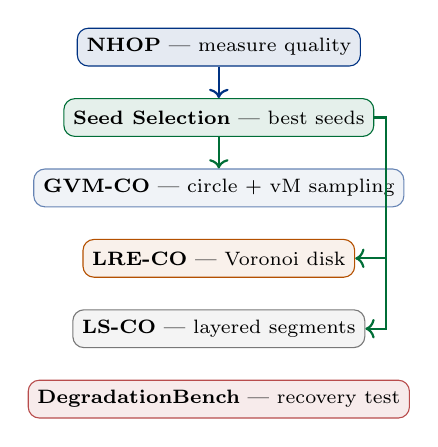
\begin{tikzpicture}[every node/.style={font=\scriptsize}, node distance=0.40cm]
  \node[draw=myblue,fill=myblue!10,rounded corners,minimum width=3.3cm,
        minimum height=0.48cm,align=center] (nhop)
    {\textbf{NHOP} — measure quality};
  \node[draw=mygreen,fill=mygreen!10,rounded corners,minimum width=3.3cm,
        minimum height=0.48cm,align=center,below=of nhop] (seed)
    {\textbf{Seed Selection} — best seeds};
  \node[draw=myblue!60,fill=myblue!6,rounded corners,minimum width=3.3cm,
        minimum height=0.48cm,align=center,below=of seed] (gvm)
    {\textbf{GVM-CO} — circle + vM sampling};
  \node[draw=myorange,fill=myorange!8,rounded corners,minimum width=3.3cm,
        minimum height=0.48cm,align=center,below=of gvm] (lre)
    {\textbf{LRE-CO} — Voronoi disk};
  \node[draw=mygray,fill=mygray!8,rounded corners,minimum width=3.3cm,
        minimum height=0.48cm,align=center,below=of lre] (ls)
    {\textbf{LS-CO} — layered segments};
  \node[draw=myred!70,fill=myred!8,rounded corners,minimum width=3.3cm,
        minimum height=0.48cm,align=center,below=of ls] (deg)
    {\textbf{DegradationBench} — recovery test};
  \draw[->,myblue,thick] (nhop)--(seed);
  \draw[->,mygreen,thick] (seed)--(gvm);
  \draw[->,mygreen,thick] (seed.east) -- ++(0.15,0)
        |- ([xshift=0.15cm]lre.east) -- (lre.east);
  \draw[->,mygreen,thick] (seed.east) -- ++(0.15,0)
        |- ([xshift=0.15cm]ls.east)  -- (ls.east);
\end{tikzpicture}
\end{columns}
\end{frame}

% ============================================================
% SLIDE 2 — Install and Quick API
% ============================================================
\begin{frame}[t,fragile]{Install \& Quick Start}
\begin{columns}[T]
\column{0.48\textwidth}
{\small\bfseries\color{myblue}Install}\\[2pt]
\begin{lstlisting}
pip install circover
\end{lstlisting}
\vspace{3pt}
{\small\bfseries\color{myblue}Measure distribution fidelity (NHOP)}\\[2pt]
\begin{lstlisting}
import circover as cc
import numpy as np

nhop = cc.NHOP(n_bins=30)

# Overall score: 1.0 = perfect, 0.0 = disjoint
score = nhop.score(X_original, X_synthetic)

# Per-feature breakdown
per_feat = nhop.score_per_feature(X_orig, X_synth)
tv_dist  = nhop.tv_per_feature(X_orig, X_synth)
# TV = 1 - NHOP  (exact identity)
\end{lstlisting}

\column{0.48\textwidth}
{\small\bfseries\color{myblue}Oversample (drop-in for SMOTE)}\\[2pt]
\begin{lstlisting}
from imblearn.pipeline import Pipeline
from sklearn.ensemble import RandomForestClassifier
from sklearn.model_selection import cross_val_score

pipe = Pipeline([
    ("over", cc.GVMCO(random_state=42)),
    # swap for: LRECO(), LSCO()
    ("clf",  RandomForestClassifier()),
])
scores = cross_val_score(
    pipe, X, y, scoring="f1", cv=5)
\end{lstlisting}
\vspace{3pt}
{\small\bfseries\color{myblue}Seed selection}\\[2pt]
\begin{lstlisting}
sel = cc.GeometricSeedSelector(
          n_seeds=20, random_state=42)
seed_idx, best_score = sel.select(X_minority)
\end{lstlisting}
\end{columns}
\end{frame}

% ============================================================
% SLIDE 3 — NHOP Intuition: 1-D bin overlap (3 cases)
% ============================================================
\begin{frame}[t]{NHOP Intuition: Shared Histogram Bins (1-D)}
\vspace{-2pt}
\begin{columns}[T]

%--- Case 1: identical ---
\column{0.32\textwidth}
\begin{center}
{\small\bfseries\color{mygreen}$\NHOP = 1.0$ — Identical}\\[2pt]
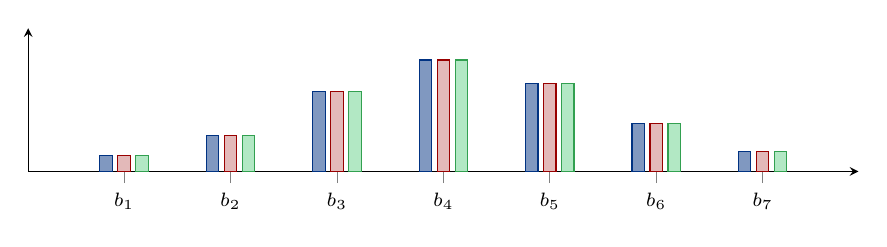
\begin{tikzpicture}
\begin{axis}[cc bar, width=\linewidth, height=3.4cm,
  ymin=0, ymax=0.36,
  xtick={1,2,3,4,5,6,7},
  xticklabels={$b_1$,$b_2$,$b_3$,$b_4$,$b_5$,$b_6$,$b_7$},
  ytick=\empty,
  bar width=4.5pt]
% P
\addplot[fill=myblue!50,draw=myblue]
  coordinates{(1,0.04)(2,0.09)(3,0.20)(4,0.28)(5,0.22)(6,0.12)(7,0.05)};
% Q (same as P, plotted slightly offset via bar width trick — use same coords)
\addplot[fill=myred!50,draw=myred,fill opacity=0.55]
  coordinates{(1,0.04)(2,0.09)(3,0.20)(4,0.28)(5,0.22)(6,0.12)(7,0.05)};
% overlap = min = same, shown green
\addplot[fill=mygreenlight,draw=mygreenbright,fill opacity=0.9]
  coordinates{(1,0.04)(2,0.09)(3,0.20)(4,0.28)(5,0.22)(6,0.12)(7,0.05)};
\end{axis}
\end{tikzpicture}\\[1pt]
{\tiny $\sum\min(p_b,q_b)=1.00$}
\end{center}

%--- Case 2: partial ---
\column{0.32\textwidth}
\begin{center}
{\small\bfseries\color{myorange}$\NHOP \approx 0.57$ — Partial}\\[2pt]
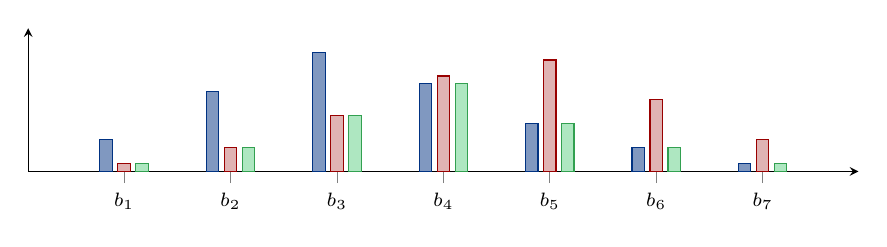
\begin{tikzpicture}
\begin{axis}[cc bar, width=\linewidth, height=3.4cm,
  ymin=0, ymax=0.36,
  xtick={1,2,3,4,5,6,7},
  xticklabels={$b_1$,$b_2$,$b_3$,$b_4$,$b_5$,$b_6$,$b_7$},
  ytick=\empty,
  bar width=4.5pt]
% P — left-shifted
\addplot[fill=myblue!50,draw=myblue]
  coordinates{(1,0.08)(2,0.20)(3,0.30)(4,0.22)(5,0.12)(6,0.06)(7,0.02)};
% Q — right-shifted
\addplot[fill=myred!50,draw=myred,fill opacity=0.6]
  coordinates{(1,0.02)(2,0.06)(3,0.14)(4,0.24)(5,0.28)(6,0.18)(7,0.08)};
% overlap = min(P,Q)
\addplot[fill=mygreenlight,draw=mygreenbright,fill opacity=0.95]
  coordinates{(1,0.02)(2,0.06)(3,0.14)(4,0.22)(5,0.12)(6,0.06)(7,0.02)};
\end{axis}
\end{tikzpicture}\\[1pt]
{\tiny $\sum\min(p_b,q_b)=0.64$\quad(scaled $\approx0.57$)}
\end{center}

%--- Case 3: disjoint ---
\column{0.32\textwidth}
\begin{center}
{\small\bfseries\color{myred}$\NHOP = 0.0$ — Disjoint}\\[2pt]
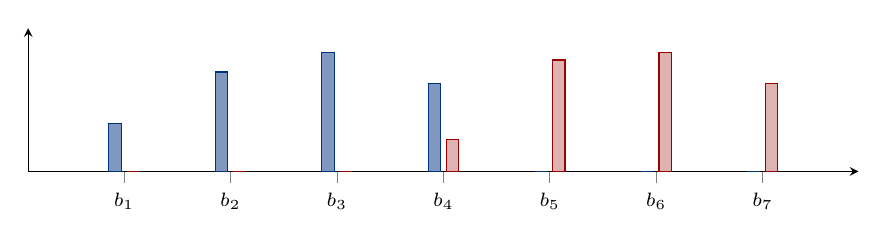
\begin{tikzpicture}
\begin{axis}[cc bar, width=\linewidth, height=3.4cm,
  ymin=0, ymax=0.36,
  xtick={1,2,3,4,5,6,7},
  xticklabels={$b_1$,$b_2$,$b_3$,$b_4$,$b_5$,$b_6$,$b_7$},
  ytick=\empty,
  bar width=4.5pt]
% P — only left bins
\addplot[fill=myblue!50,draw=myblue]
  coordinates{(1,0.12)(2,0.25)(3,0.30)(4,0.22)(5,0.0)(6,0.0)(7,0.0)};
% Q — only right bins
\addplot[fill=myred!50,draw=myred,fill opacity=0.6]
  coordinates{(1,0.0)(2,0.0)(3,0.0)(4,0.08)(5,0.28)(6,0.30)(7,0.22)};
% no overlap
\end{axis}
\end{tikzpicture}\\[1pt]
{\tiny $\sum\min(p_b,q_b)=0.00$}
\end{center}

\end{columns}
\vspace{4pt}
\begin{center}
{\footnotesize\color{mygray}
  \tikz{\fill[myblue!50](0,0)rectangle(0.28,0.11);}\;$P$ (original)\quad
  \tikz{\fill[myred!50] (0,0)rectangle(0.28,0.11);}\;$Q$ (synthetic)\quad
  \tikz{\fill[mygreenlight](0,0)rectangle(0.28,0.11);}\;$\min(p_b,q_b)$ — shared mass
}\\[2pt]
{\small\color{myblue}
  $\displaystyle\NHOP = \sum_{b=1}^{B}\min(p_b,\,q_b)$
  \quad where bins are computed on the \textit{joint} range of $P$ and $Q$}
\end{center}
\end{frame}

% ============================================================
% SLIDE 4 — NHOP Intuition: Multi-Dimensional (per feature)
% ============================================================
\begin{frame}[t]{NHOP Intuition: Multiple Dimensions}
\begin{columns}[T]
\column{0.60\textwidth}
{\small\bfseries\color{myblue}Each feature gets its own histogram overlap score}\\[3pt]
{\footnotesize
  Example: synthetic patient data ($k=3$ features).
  NHOP computed \textbf{independently} on each feature's histogram.}\\[4pt]

\begin{columns}[T]
\column{0.33\textwidth}
{\tiny\bfseries\color{myblue}Feature 1: Age}\\[1pt]
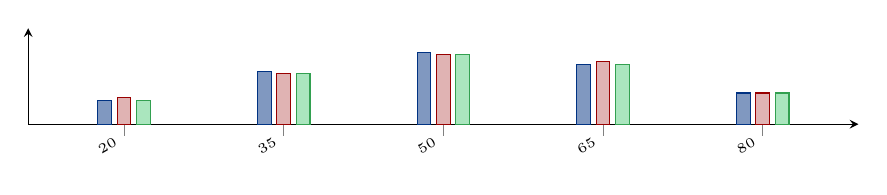
\begin{tikzpicture}
\begin{axis}[cc bar, width=\linewidth, height=2.8cm,
  ymin=0, ymax=0.40,
  xtick={1,2,3,4,5}, xticklabels={20,35,50,65,80},
  x tick label style={font=\tiny,rotate=30,anchor=east},
  ytick=\empty, bar width=5pt]
\addplot[fill=myblue!50,draw=myblue]
  coordinates{(1,0.10)(2,0.22)(3,0.30)(4,0.25)(5,0.13)};
\addplot[fill=myred!50,draw=myred,fill opacity=0.6]
  coordinates{(1,0.11)(2,0.21)(3,0.29)(4,0.26)(5,0.13)};
\addplot[fill=mygreenlight,draw=mygreenbright]
  coordinates{(1,0.10)(2,0.21)(3,0.29)(4,0.25)(5,0.13)};
\end{axis}
\end{tikzpicture}
{\tiny\color{mygreen}$\NHOP_1 = 0.98$}

\column{0.33\textwidth}
{\tiny\bfseries\color{myblue}Feature 2: BMI}\\[1pt]
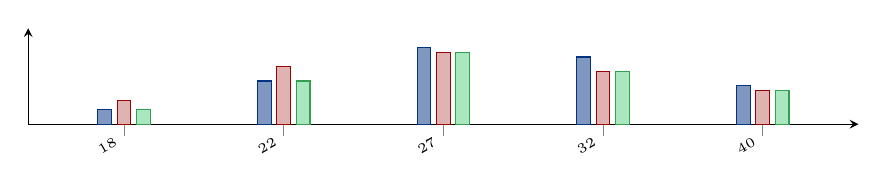
\begin{tikzpicture}
\begin{axis}[cc bar, width=\linewidth, height=2.8cm,
  ymin=0, ymax=0.40,
  xtick={1,2,3,4,5}, xticklabels={18,22,27,32,40},
  x tick label style={font=\tiny,rotate=30,anchor=east},
  ytick=\empty, bar width=5pt]
\addplot[fill=myblue!50,draw=myblue]
  coordinates{(1,0.06)(2,0.18)(3,0.32)(4,0.28)(5,0.16)};
\addplot[fill=myred!50,draw=myred,fill opacity=0.6]
  coordinates{(1,0.10)(2,0.24)(3,0.30)(4,0.22)(5,0.14)};
\addplot[fill=mygreenlight,draw=mygreenbright]
  coordinates{(1,0.06)(2,0.18)(3,0.30)(4,0.22)(5,0.14)};
\end{axis}
\end{tikzpicture}
{\tiny\color{myorange}$\NHOP_2 = 0.90$}

\column{0.33\textwidth}
{\tiny\bfseries\color{myblue}Feature 3: Glucose}\\[1pt]
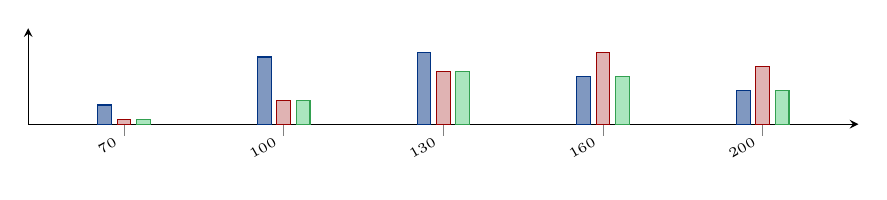
\begin{tikzpicture}
\begin{axis}[cc bar, width=\linewidth, height=2.8cm,
  ymin=0, ymax=0.40,
  xtick={1,2,3,4,5}, xticklabels={70,100,130,160,200},
  x tick label style={font=\tiny,rotate=30,anchor=east},
  ytick=\empty, bar width=5pt]
\addplot[fill=myblue!50,draw=myblue]
  coordinates{(1,0.08)(2,0.28)(3,0.30)(4,0.20)(5,0.14)};
\addplot[fill=myred!50,draw=myred,fill opacity=0.6]
  coordinates{(1,0.02)(2,0.10)(3,0.22)(4,0.30)(5,0.24)};  % shifted right
\addplot[fill=mygreenlight,draw=mygreenbright]
  coordinates{(1,0.02)(2,0.10)(3,0.22)(4,0.20)(5,0.14)};
\end{axis}
\end{tikzpicture}
{\tiny\color{myred}$\NHOP_3 = 0.68$}
\end{columns}

\vspace{6pt}
{\small\bfseries\color{myblue}Global NHOP = average over features:}\\[2pt]
{\footnotesize
$\displaystyle\NHOP = \frac{1}{3}(0.98 + 0.90 + 0.68) = \mathbf{0.853}$
}

\column{0.37\textwidth}
{\small\bfseries\color{myblue}What this tells you}\\[4pt]
{\footnotesize
\begin{tabular}{@{}lp{2.5cm}@{}}
\toprule
Feature & Diagnosis \\
\midrule
Age & $0.98$ — near-perfect \\
BMI & $0.90$ — small drift \\
Glucose & $0.68$ — \textbf{poor!} \\
\bottomrule
\end{tabular}
}\\[6pt]
{\footnotesize
\textbf{Actionable:} the oversampler distorted the Glucose distribution.
You can now \emph{target} that feature for tuning.}\\[6pt]

{\small\bfseries\color{myblue}Per-feature in code:}\\[2pt]
{\scriptsize\ttfamily\color{myblue}
\begin{tabular}{@{}l@{}}
nhop = cc.NHOP(n\_bins=30)\\
pf = nhop.score\_per\_feature(\\
\quad\quad X\_orig, X\_synth)\\
\# array([0.98, 0.90, 0.68])
\end{tabular}
}
\end{columns}
\end{frame}

% ============================================================
% SLIDE 5 — NHOP: When to Use It (intuitive use cases)
% ============================================================
\begin{frame}[t,fragile]{NHOP: When and How to Use It}
\begin{columns}[T]
\column{0.48\textwidth}
{\small\bfseries\color{myblue}1 — Did my oversampler preserve distributions?}\\[1pt]
\begin{lstlisting}
import circover as cc
nhop = cc.NHOP(n_bins=30)
X_res, _ = cc.GVMCO().fit_resample(X, y)
X_synth = X_res[len(X):]          # synthetic part
print(nhop.score(X[y==1], X_synth))
# 0.91  -- GVM-CO preserves distribution well
\end{lstlisting}
\vspace{1pt}
{\small\bfseries\color{myblue}2 — Which oversampler has better fidelity?}\\[1pt]
\begin{lstlisting}
from imblearn.over_sampling import SMOTE
smote = SMOTE().fit_resample(X, y)
X_sm  = smote[0][len(X):]
X_gvm = cc.GVMCO().fit_resample(X,y)[0][len(X):]
print(nhop.score(X[y==1], X_sm))   # 0.77
print(nhop.score(X[y==1], X_gvm))  # 0.91 better
\end{lstlisting}
{\small\bfseries\color{myblue}3 — Which features drift most?}\\[1pt]
\begin{lstlisting}
pf = nhop.score_per_feature(X[y==1], X_gvm)
# array([0.98, 0.90, 0.68])  <- feature 3 bad!
import matplotlib.pyplot as plt
plt.bar(range(len(pf)), pf)
plt.axhline(0.9, color='red', ls='--')
plt.show()
\end{lstlisting}

\column{0.48\textwidth}
{\small\bfseries\color{myblue}4 — Use NHOP as a CV scorer}\\[1pt]
\begin{lstlisting}
from sklearn.model_selection import cross_val_score

def nhop_scorer(est, X, y):
    X_r, _ = est['over'].fit_resample(X, y)
    return cc.NHOP().score(X[y==1], X_r[len(X):])

cv_nhop = cross_val_score(
    pipe, X, y, scoring=nhop_scorer, cv=5)
print(cv_nhop.mean())   # fidelity across folds
\end{lstlisting}
\vspace{3pt}
{\small\bfseries\color{myblue}5 — TV distance per feature}\\[1pt]
\begin{lstlisting}
# TV = 1 - NHOP  (exact identity, Theorem 4.5)
tv = nhop.tv_per_feature(X[y==1], X_gvm)
# array([0.02, 0.10, 0.32])
# Feature 3 has 32% TV distance -> investigate
\end{lstlisting}
\vspace{3pt}
{\small\bfseries\color{myblue}Rule of thumb}\\[2pt]
{\footnotesize
\begin{tabular}{@{}lp{2.6cm}@{}}
$\NHOP > 0.90$ & excellent fidelity \\
$0.75$--$0.90$ & acceptable \\
$< 0.75$       & distribution distorted \\
\end{tabular}
}
\end{columns}
\end{frame}

% ============================================================
% SLIDE 6 — NHOP Formal Definition
% ============================================================
\begin{frame}[t]{NHOP: Formal Definition}
\begin{columns}[T]
\column{0.54\textwidth}
{\small\bfseries\color{myblue}Definition (Normalised Histogram Overlap Percentage)}\\[3pt]
{\footnotesize
Let $X=\{x_1,\ldots,x_n\}$ and $X'=\{x'_1,\ldots,x'_m\}$ in $\mathbb{R}^k$.

For feature $j$, form the \textbf{joint} range $[\ell_j, u_j]$ over both sets.
Divide into $B$ equal-width bins. Let $p_b^j$, $q_b^j$ be normalised frequencies.

\vspace{3pt}
\textbf{Per-feature:}
\[
  \NHOP_j(X,X') \;=\; \sum_{b=1}^{B}\min\!\bigl(p_b^j,\,q_b^j\bigr) \;\in\; [0,1]
\]

\textbf{Global (mean over features):}
\[
  \NHOP(X,X') \;=\; \frac{1}{k}\sum_{j=1}^{k}\NHOP_j(X,X')
\]

\textbf{TV Identity (Theorem 4.5):}
\[
  \boxed{\NHOP_j = 1 - \TV(P^j,Q^j)}
\]
where $\TV(P,Q)=\tfrac{1}{2}\sum_b|p_b-q_b|$.
}

\column{0.43\textwidth}
\vspace{0.1cm}
{\small\bfseries\color{myblue}Why \textit{joint} normalisation?}\\[3pt]
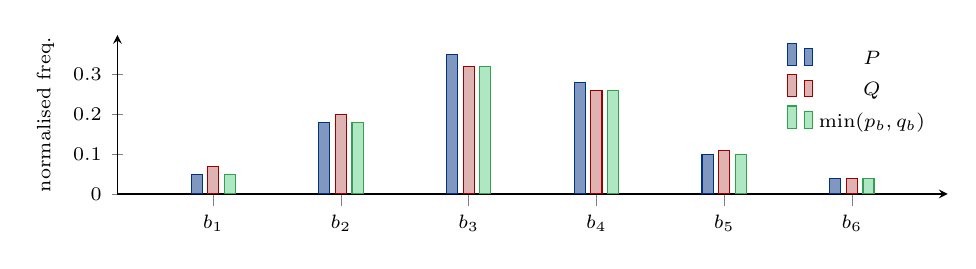
\begin{tikzpicture}
\begin{axis}[cc bar, width=\linewidth, height=3.6cm,
  ymin=0, ymax=0.40,
  ylabel={normalised freq.},
  xtick={1,2,3,4,5,6},
  xticklabels={$b_1$,$b_2$,$b_3$,$b_4$,$b_5$,$b_6$},
  ytick={0,0.1,0.2,0.3},
  bar width=4pt,
  legend style={at={(0.99,0.99)},anchor=north east}]
\addplot[fill=myblue!50,draw=myblue]
  coordinates{(1,0.05)(2,0.18)(3,0.35)(4,0.28)(5,0.10)(6,0.04)};
\addplot[fill=myred!50,draw=myred,fill opacity=0.6]
  coordinates{(1,0.07)(2,0.20)(3,0.32)(4,0.26)(5,0.11)(6,0.04)};
\addplot[fill=mygreenlight,draw=mygreenbright,fill opacity=0.95]
  coordinates{(1,0.05)(2,0.18)(3,0.32)(4,0.26)(5,0.10)(6,0.04)};
\legend{$P$,$Q$,{$\min(p_b,q_b)$}}
\end{axis}
\end{tikzpicture}
{\scriptsize\color{mygray}
  $\NHOP = 0.05+0.18+0.32+0.26+0.10+0.04 = 0.95$\\[2pt]
  Joint range: both $P$ and $Q$ map to the \textbf{same} bins,
  so $\min$ is a valid comparison.}
\end{columns}
\end{frame}

% ============================================================
% SLIDE 7 — NHOP Properties + TV identity
% ============================================================
\begin{frame}[t]{NHOP: Mathematical Properties}
\begin{columns}[T]
\column{0.50\textwidth}
{\small\bfseries\color{myblue}Analytical Properties}\\[3pt]
{\footnotesize
\begin{tabular}{@{}lp{4.2cm}@{}}
\toprule
Property & Statement \\
\midrule
Boundedness & $\NHOP \in [0,1]$ always \\
Symmetry & $\NHOP(X,X') = \NHOP(X',X)$ \\
Identity & $X=X' \Rightarrow \NHOP = 1$ \\
Disjoint & $\mathrm{supp}(P)\cap\mathrm{supp}(Q)=\emptyset \Rightarrow 0$ \\
Scale inv. & invariant to affine rescaling of features \\
\bottomrule
\end{tabular}
}\\[5pt]

{\small\bfseries\color{myred}TV Identity — Proof Sketch}\\[3pt]
{\footnotesize
Since $\sum_b p_b = \sum_b q_b = 1$:
\[
  \sum_b \min(p_b,q_b) = 1 - \sum_b \max(p_b-q_b,\,0)
  = 1 - \tfrac{1}{2}\sum_b|p_b-q_b|
\]
The last equality holds because $\sum_b(p_b-q_b)=0$.
Hence $\NHOP_j = 1 - \TV(P^j,Q^j)$. \hfill$\square$
}

\column{0.47\textwidth}
\vspace{0.1cm}
{\small\bfseries\color{myblue}NHOP and TV are exact complements}\\[3pt]
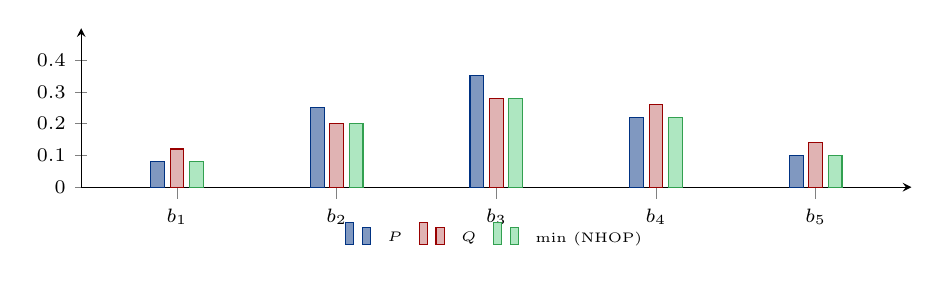
\begin{tikzpicture}
\begin{axis}[cc bar, width=\linewidth, height=3.6cm,
  ymin=0, ymax=0.50,
  xtick={1,2,3,4,5},
  xticklabels={$b_1$,$b_2$,$b_3$,$b_4$,$b_5$},
  ytick={0,0.1,0.2,0.3,0.4},
  bar width=5pt,
  legend style={at={(0.5,-0.18)},anchor=north,font=\tiny,
                legend columns=3,column sep=4pt}]
% P
\addplot[fill=myblue!50,draw=myblue]
  coordinates{(1,0.08)(2,0.25)(3,0.35)(4,0.22)(5,0.10)};
% Q
\addplot[fill=myred!50,draw=myred,fill opacity=0.6]
  coordinates{(1,0.12)(2,0.20)(3,0.28)(4,0.26)(5,0.14)};
% min (NHOP part)
\addplot[fill=mygreenlight,draw=mygreenbright,fill opacity=0.95]
  coordinates{(1,0.08)(2,0.20)(3,0.28)(4,0.22)(5,0.10)};
\legend{$P$,$Q$,{$\min$~(NHOP)}}
\end{axis}
\end{tikzpicture}
{\scriptsize\color{mygray}
  Green area $= \NHOP = 0.88$.\quad
  Remaining (blue+red not covered) $= \TV = 0.12$.\quad
  $\NHOP + \TV = 1.0$.}
\end{columns}
\end{frame}

% ============================================================
% SLIDE 8 — Geometry-Preserving Seed Selection
% ============================================================
\begin{frame}[t]{Geometry-Preserving Seed Selection}
\begin{columns}[T]
\column{0.52\textwidth}
{\small\bfseries\color{myblue}Problem}\\[1pt]
{\footnotesize
Standard oversamplers use every point as a seed — including
noisy outliers that distort synthesis.
}\\[2pt]
{\small\bfseries\color{myblue}Composite Score}\\[1pt]
{\footnotesize
\[
  S(C) = \NHOP(C) + \mathrm{AGTP}(C)
        - w_J\,\mathrm{JSD}(C) - w_Z\,Z(C)
\]
}
{\scriptsize
\begin{tabular}{@{}lp{3.8cm}@{}}
\toprule
Term & Meaning \\
\midrule
$\NHOP(C)$ & histogram overlap: seed set $C$ vs.\ full minority \\
$\mathrm{AGTP}=G_\text{sim}+T_\text{sim}$ & geometry + topology match \\
$\mathrm{JSD}(C)$ & Jensen-Shannon penalty (divergence) \\
$Z(C) = \sigma/\mu$ of nn-dists & spacing regularity penalty \\
\bottomrule
\end{tabular}
}\\[4pt]
{\small\bfseries\color{mygreen}Impact}\\[1pt]
{\scriptsize\begin{tabular}{@{}lc@{}}
\toprule Seeds & NHOP \\ \midrule
Random & 0.766 \\
\textbf{Geometric} & \textbf{0.907} \\
\bottomrule
\end{tabular}}

\column{0.45\textwidth}
{\small\bfseries\color{myblue}4-Stage Pipeline}\\[1pt]
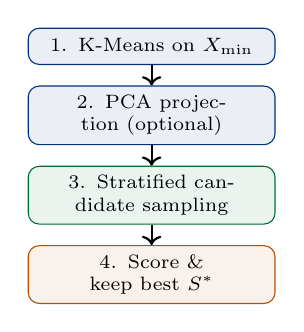
\begin{tikzpicture}[node distance=0.26cm, every node/.style={font=\scriptsize}]
  \node[draw=myblue,fill=myblue!8,rounded corners,text width=2.9cm,
        align=center,minimum height=0.46cm] (km)
    {1. K-Means on $X_\text{min}$};
  \node[draw=myblue,fill=myblue!8,rounded corners,text width=2.9cm,
        align=center,minimum height=0.46cm,below=of km] (pca)
    {2. PCA projection (optional)};
  \node[draw=mygreen,fill=mygreen!8,rounded corners,text width=2.9cm,
        align=center,minimum height=0.46cm,below=of pca] (samp)
    {3. Stratified candidate sampling};
  \node[draw=myorange,fill=myorange!8,rounded corners,text width=2.9cm,
        align=center,minimum height=0.46cm,below=of samp] (score)
    {4. Score \& keep best $S^*$};
  \draw[->,thick] (km)--(pca);
  \draw[->,thick] (pca)--(samp);
  \draw[->,thick] (samp)--(score);
\end{tikzpicture}
\vspace{2pt}
{\small\bfseries\color{myblue}Code}\\[1pt]
{\scriptsize\ttfamily\color{myblue}
sel = cc.GeometricSeedSelector(\\
\quad\quad n\_seeds=20,\\
\quad\quad n\_candidates=100,\\
\quad\quad random\_state=42)\\
idx, score = sel.select(X\_minority)
}
\end{columns}
\end{frame}

% ============================================================
% SLIDE 9 — GVM-CO
% ============================================================
\begin{frame}[t]{GVM-CO: Gravity-Biased Von Mises Circular Oversampling}
\begin{columns}[T]
\column{0.40\textwidth}
{\small\bfseries\color{myblue}Algorithm}\\[2pt]
{\footnotesize
For each seed pair $(s_i, s_j)$ (k-NN):
\begin{enumerate}\itemsep1pt
  \item Circle: centre $m_{ij}$, radius $r_{ij}=\tfrac{1}{2}\|s_i-s_j\|$
  \item Angle: $\theta\sim\mathrm{vM}(\mu_{\text{toward }g_c},\kappa_{ij})$
  \item New point: $x'=m_{ij}+r_{ij}(\cos\theta,\sin\theta)$
\end{enumerate}
}\\[3pt]
{\small\bfseries\color{myblue}Gravity concentration}\\[2pt]
{\footnotesize
$g_c = \rho_c/(\sigma_c\cdot\bar{d}_c)$,\quad
$s_{ij} = \alpha\tilde{g}_c + (1{-}\alpha)(1{-}\bar{d}_{ij}/d_\text{max})$\\[2pt]
$\kappa_{ij} = \kappa_\text{max}\cdot s_{ij}^{\,\gamma}$\quad
(high gravity $\Rightarrow$ high $\kappa$)
}\\[3pt]
{\scriptsize\ttfamily\color{myblue}
cc.GVMCO(n\_clusters=5,\\
\quad kappa\_max=4.0, random\_state=42)
}

\column{0.57\textwidth}
\begin{center}
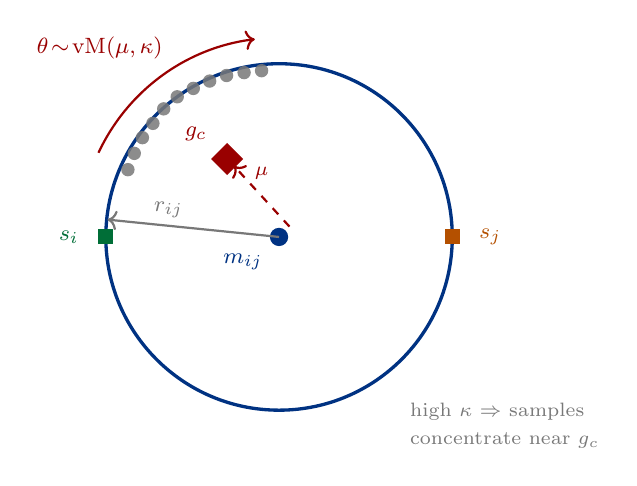
\begin{tikzpicture}[scale=1.1, every node/.style={font=\footnotesize}]
  % --- circle ---
  \draw[myblue, very thick] (0,0) circle (2cm);
  % --- midpoint ---
  \fill[myblue] (0,0) circle (3pt);
  \node[myblue, anchor=north east] at (-0.08,-0.08) {$m_{ij}$};
  % --- radius arrow (left side, clear of labels) ---
  \draw[->,thick,mygray] (0,0) -- (-1.98,0.2)
    node[midway, above left, mygray] {$r_{ij}$};
  % --- seed s_i (left) ---
  \node[draw=mygreen,fill=mygreen,inner sep=2.5pt,rectangle] at (-2,0) {};
  \node[mygreen, anchor=east] at (-2.2,0) {$s_i$};
  % --- seed s_j (right) ---
  \node[draw=myorange,fill=myorange,inner sep=2.5pt,rectangle] at (2,0) {};
  \node[myorange, anchor=west] at (2.2,0) {$s_j$};
  % --- gravity center (upper-left inside circle, off-axis for visual clarity) ---
  \node[draw=myred,fill=myred,inner sep=2.8pt,diamond] at (-0.6,0.9) {};
  \node[myred, anchor=south east] at (-0.72,1.0) {$g_c$};
  % --- dashed arrow from m_ij toward g_c (shows Von Mises mean direction) ---
  \draw[->,myred,dashed,thick] (0.12,0.12) -- (-0.52,0.82);
  \node[myred, anchor=south, font=\scriptsize] at (-0.2,0.55) {$\mu$};
  % --- sample points clustered near g_c on the circle (~120 deg) ---
  \foreach \a/\r in {120/1.98, 126/2.00, 132/1.99, 114/1.97,
                     138/1.96, 108/1.96, 144/1.95, 102/1.94,
                     150/1.93,  96/1.93, 156/1.91}{
    \fill[mygray,opacity=0.85] ({\r*cos(\a)},{\r*sin(\a)}) circle (2.2pt);
  }
  % --- arc annotation (outside circle, near sample cluster) ---
  \draw[->,myred,thick]
    ({2.3*cos(155)},{2.3*sin(155)}) arc[start angle=155,end angle=97,radius=2.3cm];
  \node[myred, anchor=south east] at ({2.15*cos(125)},{2.15*sin(125)+0.18})
    {$\theta\!\sim\!\mathrm{vM}(\mu,\kappa)$};
  % --- note ---
  \node[mygray, anchor=north west, align=left] at (1.4,-1.8)
    {\scriptsize high $\kappa$ $\Rightarrow$ samples};
  \node[mygray, anchor=north west, align=left] at (1.4,-2.15)
    {\scriptsize concentrate near $g_c$};
\end{tikzpicture}
\end{center}
\vspace{0pt}
\end{columns}
\end{frame}

% ============================================================
% SLIDE 10 — LRE-CO
% ============================================================
\begin{frame}[t]{LRE-CO: Local Region Estimation Circular Oversampling}
\begin{columns}[T]
\column{0.40\textwidth}
{\small\bfseries\color{myblue}Key Idea}\\[2pt]
{\footnotesize
LRE-CO constrains sampling to the \textbf{Voronoi cell} of each cluster,
preventing spillover into majority territory.
}\\[2pt]
{\small\bfseries\color{myblue}Algorithm}\\[1pt]
{\footnotesize
\begin{enumerate}\itemsep1pt
  \item K-Means; compute Voronoi cells $V_c$
  \item Certainty check: $P(c\mid s_i)\ge\tau{=}0.80$
  \item Sample: $x'\sim\mathrm{Uniform}(\mathrm{disk}(s_i,r_i))$
  \item \textbf{Reject} if $x'\notin V_c$; repeat
  \item Cluster weight: $w_c\propto\tilde{g}_c\cdot n_c$
\end{enumerate}
}\\[2pt]
{\footnotesize\color{mygreen}
  \textbf{Guarantee:} all synthetic points stay in $V_c$.}\\[3pt]
{\scriptsize\ttfamily\color{myblue}
cc.LRECO(certainty\_threshold=0.80,\\
\quad random\_state=42)
}

\column{0.57\textwidth}
\begin{center}
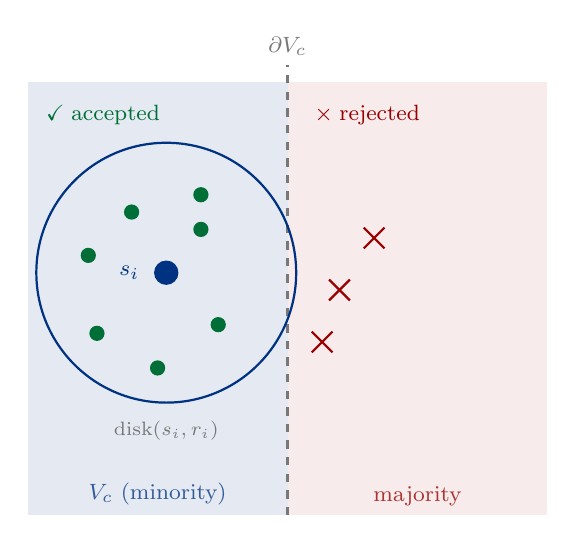
\begin{tikzpicture}[scale=1.1, every node/.style={font=\footnotesize}]
  % --- Voronoi boundary ---
  \draw[mygray,thick,dashed] (0,-2.5) -- (0,2.7);
  \node[mygray,anchor=south] at (0,2.7) {$\partial V_c$};
  % --- filled regions ---
  \fill[myblue!10] (-3,-2.5) rectangle (0,2.5);
  \fill[myred!8]   (0,-2.5) rectangle (3,2.5);
  % redraw boundary on top
  \draw[mygray,thick,dashed] (0,-2.5) -- (0,2.7);
  % region labels
  \node[myblue!80,anchor=south] at (-1.5,-2.5) {$V_c$ (minority)};
  \node[myred!80,anchor=south]  at ( 1.5,-2.5) {majority};
  % --- seed s_i ---
  \fill[myblue] (-1.4,0.3) circle (4pt);
  \node[myblue,anchor=east] at (-1.6,0.3) {$s_i$};
  % --- disk boundary ---
  \draw[myblue,thick] (-1.4,0.3) circle (1.5cm);
  \node[mygray,anchor=north] at (-1.4,-1.3) {\scriptsize disk$(s_i,r_i)$};
  % --- accepted points (inside disk AND inside Vc) ---
  \foreach \x/\y in {-1.0/1.2, -1.8/1.0, -2.3/0.5, -1.5/-0.8,
                     -0.8/-0.3, -2.2/-0.4, -1.0/0.8}{
    \fill[mygreen] (\x,\y) circle (2.5pt);
  }
  \node[mygreen,anchor=south west] at (-2.9,1.9) {\checkmark\;accepted};
  % --- rejected points (outside Vc) ---
  \foreach \x/\y in {0.6/0.1, 1.0/0.7, 0.4/-0.5}{
    \draw[myred,thick] (\x-0.12,\y-0.12) -- (\x+0.12,\y+0.12);
    \draw[myred,thick] (\x-0.12,\y+0.12) -- (\x+0.12,\y-0.12);
  }
  \node[myred,anchor=south west] at (0.2,1.9) {$\times$\;rejected};
\end{tikzpicture}
\end{center}
\vspace{0pt}
\end{columns}
\end{frame}

% ============================================================
% SLIDE 11 — LS-CO
% ============================================================
\begin{frame}[t]{LS-CO: Layered Segmental Circular Oversampling}
\begin{columns}[T]
\column{0.40\textwidth}
{\small\bfseries\color{myblue}Structure: $L$ layers $\times$ $M$ segments}\\[2pt]
{\footnotesize
Concentric rings (layers) $\times$ angular slices (segments)
around each cluster gravity center.
}\\[2pt]
{\small\bfseries\color{myblue}Mathematics}\\[1pt]
{\footnotesize
\textbf{Layer weight:}\\
$w_\ell \propto \exp\!\bigl(-\tfrac{(\ell-\ell^*)^2}{2\sigma_L^2}\bigr)\cdot\tilde{g}_c$\\[3pt]
\textbf{Segment concentration:}\\
$\kappa_s = \kappa_\text{max}\cdot(n_s/n_\text{layer})^{\gamma}$\\[3pt]
\textbf{Area-uniform radius:}\\
$r = \sqrt{r_\text{in}^2 + u(r_\text{out}^2-r_\text{in}^2)},\;u\sim U[0,1]$
}\\[3pt]
{\scriptsize\ttfamily\color{myblue}
cc.LSCO(n\_layers=3, n\_segments=6,\\
\quad kappa\_max=4.0, random\_state=42)
}

\column{0.57\textwidth}
\begin{center}
{\scriptsize\color{myblue}\bfseries $L{=}3$ layers, $M{=}6$ segments}\\[2pt]
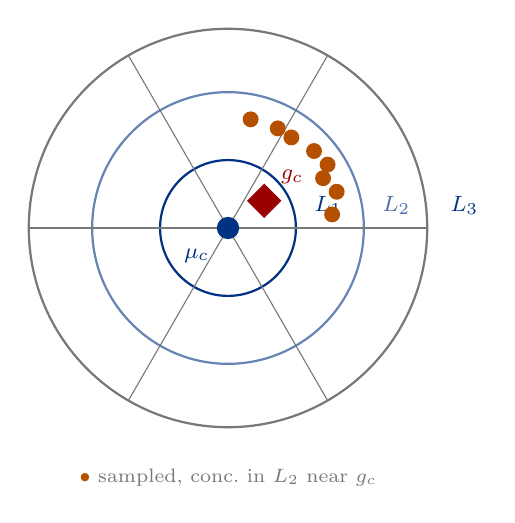
\begin{tikzpicture}[scale=1.15, every node/.style={font=\footnotesize}]
  % --- three concentric circles (L1=inner, L2=mid, L3=outer) ---
  \draw[mygray,thick]   (0,0) circle (2.2cm);   % L3 outer
  \draw[myblue!60,thick](0,0) circle (1.5cm);   % L2 mid
  \draw[myblue,thick]   (0,0) circle (0.75cm);  % L1 inner
  % --- 6 spokes (segment dividers) at 0,60,120,180,240,300 deg ---
  \foreach \a in {0,60,120,180,240,300}{
    \draw[mygray,thin] (0,0) -- ({2.2*cos(\a)},{2.2*sin(\a)});
  }
  % --- layer labels (right side, clear spacing) ---
  \node[myblue,anchor=west]    at (2.35, 0.25) {$L_3$};
  \node[myblue!70,anchor=west] at (1.60, 0.25) {$L_2$};
  \node[myblue,anchor=west]    at (0.85, 0.25) {$L_1$};
  % --- gravity center (red diamond) ---
  \node[draw=myred,fill=myred,inner sep=3pt,diamond] at (0.4,0.3) {};
  \node[myred,anchor=south west] at (0.48,0.38) {$g_c$};
  % --- cluster centroid (blue dot) ---
  \fill[myblue] (0,0) circle (3.5pt);
  \node[myblue,anchor=north east] at (-0.1,-0.12) {$\mu_c$};
  % --- sampled points (orange, concentrated in L2 first-quadrant sector) ---
  \foreach \x/\y in {0.95/0.85, 1.05/0.55, 0.55/1.10, 1.15/0.15,
                     0.25/1.20, 1.10/0.70, 0.70/1.00, 1.20/0.40}{
    \fill[myorange] (\x,\y) circle (2.5pt);
  }
  % --- legend note below ---
  \node[mygray,anchor=north] at (0,-2.55)
    {\scriptsize \textcolor{myorange}{$\bullet$} sampled, conc.\ in $L_2$ near $g_c$};
\end{tikzpicture}
\end{center}
\end{columns}
\end{frame}

% ============================================================
% SLIDE 12 — Algorithm Comparison
% ============================================================
\begin{frame}[t]{Algorithm Comparison}
\begin{columns}[T]
\column{0.48\textwidth}
{\small\bfseries\color{myblue}Summary}\\[3pt]
{\scriptsize
\begin{tabular}{@{}lp{1.7cm}p{2.0cm}@{}}
\toprule
Method & Region & Bias \\
\midrule
\textbf{GVM-CO} & circle (2 seeds) & vM toward $g_c$ \\[2pt]
\textbf{LRE-CO} & disk $\cap$ Voronoi & grav.\ cluster wt. \\[2pt]
\textbf{LS-CO} & annular layers & layer wt.\ + seg.\ $\kappa$ \\
\bottomrule
\end{tabular}
}\\[4pt]
{\small\bfseries\color{myblue}All three}\\[2pt]
{\footnotesize
\begin{itemize}\itemsep1pt
  \item Drop-in for SMOTE (imblearn API)
  \item \texttt{use\_pca=False} native-dim mode
  \item \texttt{random\_state} reproducibility
  \item sklearn CV / pipeline compatible
\end{itemize}
}

\column{0.48\textwidth}
{\small\bfseries\color{myblue}F1 comparison (14 datasets)}\\[3pt]
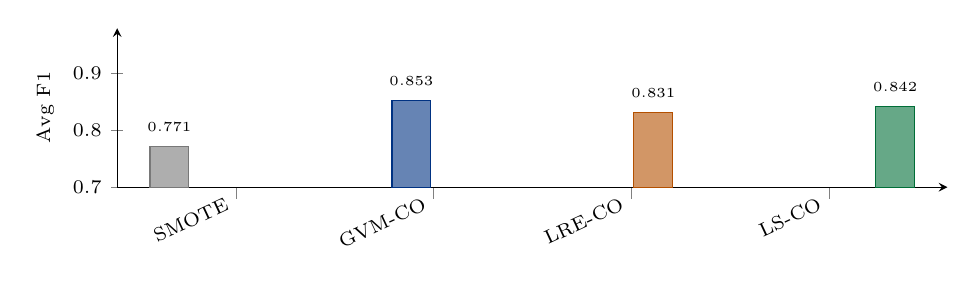
\begin{tikzpicture}
\begin{axis}[cc bar, width=\linewidth, height=3.6cm,
  ymin=0.70, ymax=0.98,
  xtick={1,2,3,4},
  xticklabels={SMOTE, GVM-CO, LRE-CO, LS-CO},
  x tick label style={font=\scriptsize,rotate=25,anchor=east},
  enlarge x limits={abs=0.6},
  ylabel={Avg F1},
  nodes near coords,
  nodes near coords style={font=\tiny,yshift=2pt},
  every node near coord/.append style={
    /pgf/number format/.cd, fixed, precision=3},
  bar width=14pt]
\addplot[fill=mygray!60,draw=mygray]    coordinates {(1,0.771)};
\addplot[fill=myblue!60,draw=myblue]    coordinates {(2,0.853)};
\addplot[fill=myorange!60,draw=myorange] coordinates {(3,0.831)};
\addplot[fill=mygreen!60,draw=mygreen]  coordinates {(4,0.842)};
\end{axis}
\end{tikzpicture}
{\scriptsize\color{mygray}
  GVM-CO achieves highest avg.\ F1; all circular methods outperform SMOTE.}
\end{columns}
\end{frame}

% ============================================================
% SLIDE 13 — Degradation Benchmark
% ============================================================
\begin{frame}[t,fragile]{Degradation-and-Recovery Benchmark}
\begin{columns}[T]
\column{0.50\textwidth}
{\small\bfseries\color{myblue}What it tests}\\[2pt]
{\footnotesize
\begin{enumerate}\itemsep1pt
  \item Remove minority samples in $\delta$ steps ($0\%\to100\%$)
  \item Apply oversampler + classifier at each level
  \item Record F1/AUC via cross-validation
  \item Compute \textbf{ARI} = $\int_0^1\mathrm{score}(\delta)\,d\delta$
\end{enumerate}
Higher ARI = better recovery from imbalance.
}\\[4pt]
\begin{lstlisting}
bench = cc.DegradationBench(
    steps=10, metric="f1",
    cv=5, random_state=42)

# Run on any pipeline
results = bench.run(pipe, X, y)
bench.plot(results)    # recovery curve
ari = cc.DegradationBench\
    .area_recovery_index(results)

# Compare methods
ari_smote = bench.run(smote_pipe, X, y)
ari_gvm   = bench.run(gvm_pipe,   X, y)
\end{lstlisting}

\column{0.47\textwidth}
\vspace{0.1cm}
{\small\bfseries\color{myblue}Recovery curves}\\[2pt]
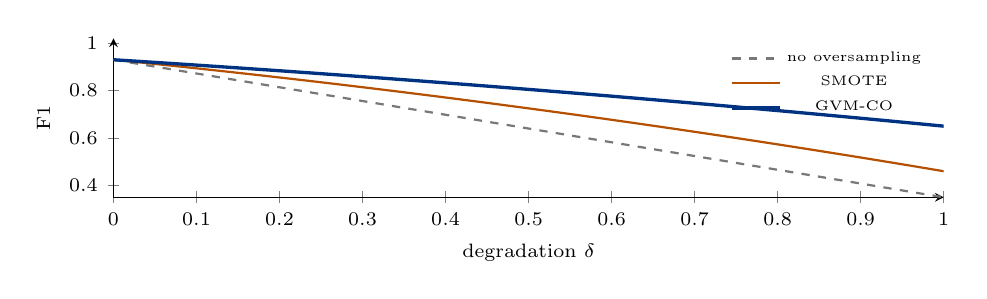
\begin{tikzpicture}
\begin{axis}[cc axis, width=\linewidth, height=3.6cm,
  domain=0:1, samples=50,
  xlabel={degradation $\delta$}, ylabel={F1},
  ymin=0.35, ymax=1.02,
  legend style={at={(0.99,0.99)},anchor=north east,font=\tiny}]
\addplot[mygray, thick, dashed]
  {max(0.35, 0.93 - 0.58*x)};
\addplot[myorange, thick]
  {max(0.35, 0.93 - 0.35*x - 0.12*x*x)};
\addplot[myblue, very thick]
  {max(0.35, 0.93 - 0.22*x - 0.06*x*x)};
\legend{no oversampling, SMOTE, GVM-CO}
\end{axis}
\end{tikzpicture}
\vspace{2pt}
{\footnotesize
\begin{tabular}{@{}lc@{}}
\toprule Method & ARI \\
\midrule
None (baseline) & 0.64 \\
SMOTE & 0.74 \\
\textbf{GVM-CO} & \textbf{0.82} \\
\bottomrule
\end{tabular}
}
\end{columns}
\end{frame}

% ============================================================
% SLIDE 14 — GitHub and Usage
% ============================================================
\begin{frame}[t,fragile]{GitHub Repository and Usage}
\begin{columns}[T]
\column{0.52\textwidth}
{\small\bfseries\color{myblue}Links}\\[1pt]
{\scriptsize
\texttt{github.com/Parsa-Hajian/circover}\quad
\texttt{pypi.org/project/circover/}
}\\[3pt]
{\small\bfseries\color{myblue}Complete workflow}\\[1pt]
\begin{lstlisting}
import circover as cc
from imblearn.pipeline import Pipeline
from sklearn.ensemble import RandomForestClassifier
from sklearn.model_selection import cross_val_score

# 1. Build pipeline (drop-in for SMOTE)
pipe = Pipeline([
    ("over", cc.GVMCO(random_state=42)),
    ("clf",  RandomForestClassifier()),
])
print(cross_val_score(pipe, X, y,
                      scoring="f1", cv=5).mean())

# 2. Check distribution fidelity
X_res, _ = pipe['over'].fit_resample(X, y)
nhop = cc.NHOP()
print(nhop.score(X[y==1], X_res[len(X):]))

# 3. Run degradation benchmark
bench = cc.DegradationBench(steps=10)
results = bench.run(pipe, X, y)
bench.plot(results)
\end{lstlisting}

\column{0.44\textwidth}
{\small\bfseries\color{myblue}Modules}\\[2pt]
{\scriptsize\begin{tabular}{@{}lp{2.6cm}@{}}
\toprule File & Export \\ \midrule
\texttt{nhop.py} & \texttt{NHOP} \\
\texttt{seed\_selection.py} & \texttt{GeometricSeedSelector} \\
\texttt{oversampling.py} & \texttt{GVMCO, LRECO, LSCO} \\
\texttt{degradation.py} & \texttt{DegradationBench} \\
\texttt{\_gravity.py} & (internal utils) \\
\bottomrule
\end{tabular}}\\[5pt]
{\small\bfseries\color{myblue}Key parameters}\\[2pt]
{\scriptsize\begin{tabular}{@{}lp{2.5cm}@{}}
\toprule Param & Meaning \\ \midrule
\texttt{n\_bins=30} & histogram bins \\
\texttt{n\_clusters=5} & K-Means clusters \\
\texttt{kappa\_max=4.0} & max vM concentration \\
\texttt{use\_pca=True} & PCA mode \\
\texttt{steps=10} & degradation steps \\
\bottomrule
\end{tabular}}\\[5pt]
{\scriptsize\color{mygreen}\textbf{16/16 tests passing}\quad
\texttt{pytest tests/}}
\end{columns}
\end{frame}

\end{document}
